\subsection{Introducción}
En la sección anterior implementamos y analizamos una heurística golosa para atacar el problema planteado. Si bien resulta bastante deseable desde el punto de vista de la complejidad temporal (polinomial de grado razonable), tiene el problema de que, como vimos, la solución que nos provee puede ser arbitrariamente mala y en el caso general no tenemos ningún tipo de garantía de qué tan cerca puede estar de una solución verdaderamente óptima.

Lo que quisiéramos entonces es poder refinar la solución que nos devuelve la heurística golosa para que se acerce más al máximo real. Para esto probaremos 3 algoritmos de búsqueda local. Dichos algoritmos se basan en la noción de ``vecindad'' de soluciones. Dada una solución fuente, una vecindad de $S$, $N(S)$, es un subconjunto del conjunto de posibles soluciones (en nuestro caso un subconjunto del conjunto de subgrafos comunes) que a diferencia de este último tiene un cardinal lo suficientemente pequeño como para poder ser recorrido en tiempo polinomial. Entonces los algoritmos de búsqueda local se diferenciarán a partir de la vecindad escogida en cada caso.

Es importante resaltar que los algoritmos de búsqueda local no dejan de ser algoritmos heurísticos cuya calidad dependerá tanto de la solución fuente utilizada como de la vecindad escogida. Los algoritmos solo nos garantizan que encontraremos el máximo de la vecindad (máximo local) que no necesariamente es el máximo global.

Otra cosa importante que también será común a todas las búsquedas es que cuando encontremos un máximo en la vecindad, si es mejor que la solución \emph{source}, no nos conformaremos con esto sino que pasaremos a explorar la vecindad correspondiente a esta nueva solución. De forma que se iterará la búsqueda hasta que se llegue a una solución que sea máxima en su vecindad.

En particular nosotros escogimos 3 vecindades para el problema, bajo los siguientes rótulos:
\begin{itemize}
	\item INTERCAMBIAR
	\item REEMPLAZAR
	\item 3-ROTACION 
\end{itemize}

En todos los casos la solución fuente inicial será la dada por el algoritmo goloso.

\subsection{Explicación detallada de los algoritmos}
En pos de la claridad separamos la explicación y el pseudocódigo de las tres vecindades. 

La notación usada será $n_1 = |V(G_1)|$, $n_2 = |V(G_2)|$, $m_1 = |E(G_1)|$ y $m_2 = |E(G_2)|$. Asumimos, por ser precondición para usar el algoritmo goloso y la heurística REMPLAZAR, que $n_1 \leq n_2$. 

\subsubsection{INTERCAMBIAR}
Un aspecto importante de nuestro algoritmo goloso es que siempre mapea exactamente todos los vértices del grafo con menor número de vértices a la hora de devolver la solución. En esta primera vecindad lo que planteamos es considerar todos los \emph{swapeos} posibles para el mapeo de la solución \emph{source}. Formalmente, si $S = \{(v_0, w_{i_1}),\hdots , (v_n, w_{i_n})\}$ es el mapeo de la solución \emph{source}, entonces la vecindad de tipo INTERCAMBIAR asociada a S es $N_I(S) = \{S' : S' = \{(v_0, w_{i_1}),\hdots , (v_p, w_{i_q}) , \hdots, (v_q, w_{i_p}), (v_n, w_{i_n})\}\}$.

\begin{algorithm}[H]
  \small
  \begin{algorithmic}[1]
  \caption{Pseudocódigo de INTERCAMBIAR}
  \label{algo:5-1}
    \Procedure{INT}{\texttt{Grafo} $G_1$, \texttt{set<int>} $vertices_1$, \texttt{Grafo} $G_2$, \texttt{set<int>} $vertices_2$}$\rightarrow$ \texttt{MCS}
      \State \texttt{MCS} $source \gets goloso(G_1, vertices_1, G_2, vertices_2)$
      \Comment $O(n_1^4n_2)$
      \State \texttt{bool} $mejore \gets true$
      \Comment $O(1)$
      \While{$mejore$}
      \Comment $O(min\{m_1, m_2\})$
        \State $mejore \gets false$
        \Comment $O(1)$
        \For{$i \gets 0 \hdots |source.isomorfismo|$}
        \Comment $n_1$ veces
          \For{$j \gets 0\hdots |source.isomorfismo|, i \neq j$}
          \Comment $n_1$ veces
            \State $swap(source.isomorfismo[i].first, source.isomorfismo[j].first)$
            \Comment $O(1)$
            \State \texttt{int} $aristas \gets contar\_aristas\_isomorfismo(G_1, G_2, source.isomorfismo)$
            \Comment $O(n_1^2)$
            \If{$aristas > source.aristas$}
            \Comment $O(1)$
              \State $source.aristas \gets aristas$ 
              \Comment $O(1)$             
              \State $mejore \gets true$
              \Comment $O(1)$
            \EndIf
          \EndFor
        \EndFor
      \EndWhile
    \EndProcedure
  \end{algorithmic}
  Complejidad: $O(min{n_1, n_2})$
\end{algorithm}

\subsubsection{REEMPLAZAR}
Recordar que $n_1 \leq n_2$ por precondición. En particular, para esta vecindad solo nos interesarán los casos en que $n_1 < n_2$. Si ambos tamaños fueran iguales el algoritmo no modificará la solución golosa.

Debido a esta condición extra que asumimos sobre el tamaño de los grafos, para cualquier mapeo que tengamos como solución (en particular, el dado por el algoritmo goloso) siempre hay vértices de $G_2$ que no se están mapeando.

La motivación de esta vecindad entonces es ver qué sucede con la cantidad de aristas cuando en el mapeo de la solución fuente reemplazamos nodos de $G_2$ con otros que no habíamos usado originalmente.

Formalmente, si $S = \{(v_0, w_{1}),\hdots , (v_n, w_{n})\}$ es el mapeo de la solución fuente y $R = \{z_1, \hdots, z_r\}$ son los vértices de $G_2$ que no se mapearon en $S$, entonces \\
$N(S) = \{S': S' = S \textbackslash \{(v_i, w_i)\} \cup \{(v_i, z_i)\}\}$. 

\begin{algorithm}[H]
  \small
  \begin{algorithmic}[1]
  \caption{Pseudocódigo de REMPLAZAR}
  \label{algo:5-2}
    \Procedure{REMP}{\texttt{Grafo} $G_1$, \texttt{set<int>} $vertices_1$, \texttt{Grafo} $G_2$, \texttt{set<int>} $vertices_2$}$\rightarrow$ \texttt{MCS}
      \State \texttt{MCS} $source \gets goloso(G_1, vertices_1, G_2, vertices_2)$
      \Comment $O(n_1^4n_2)$
      \State \texttt{bool} $mejore \gets true$
      \Comment $O(1)$
      \State \texttt{vector<int>} $vertices \gets set\_to\_vector(vertices_2)$
      \Comment $O(n_2-n_1)$
      \While{$mejore$}
      \Comment $O(min\{m_1, m_2\})$
        \State $mejore \gets false$
        \Comment $O(1)$
        \For{$i \gets 0 \hdots |vertices|$}
        \Comment $n_2-n_1$ veces
          \For{$j \gets 0 \hdots |source.isomorfismo|$}
          \Comment $n_1$ veces
            \State $swap(vertices[i], source.isomorfismo[j].second)$
            \Comment $O(1)$
            \State \texttt{int} $aristas \gets contar\_aristas\_isomorfismo(G_1, G_2, source.isomorfismo)$
            \Comment $O(n_1^2)$
            \If{$aristas > source.aristas$}
            \Comment $O(1)$
              \State $source.aristas \gets aristas$  
              \Comment $O(1)$            
              \State $mejore \gets true$
              \Comment $O(1)$
            \Else
              \State $swap(vertices[i], source.isomorfismo[j].second)$
              \Comment $O(1)$
            \EndIf
          \EndFor
        \EndFor
      \EndWhile
    \EndProcedure
  \end{algorithmic}
\end{algorithm}

\subsubsection{3-ROTACION}
Esta vecindad sigue un principio muy parecido al de INTERCAMBIAR. La idea surge por analogía de las búsquedas locales 2-opt y 3-opt vistas en la teórica. En INTERCAMBIAR solo considerábamos como vecindad las soluciones que estaban a un \emph{swap} de diferencia del mapeo fuente. En ese caso los \emph{swapeos} pueden considerarse como una rotación de solo dos elementos. En esta variación la vecindad estará compuesta por todas las soluciones que están a lo sumo a una rotación de 3 nodos de diferencia.

\begin{algorithm}[H]
  \small
  \begin{algorithmic}[1]
  \caption{Pseudocódigo de 3-ROTACION}
  \label{algo:5-3}
    \Procedure{3-ROT}{\texttt{Grafo} $G_1$, \texttt{set<int>} $vertices_1$, \texttt{Grafo} $G_2$, \texttt{set<int>} $vertices_2$}$\rightarrow$ \texttt{MCS}
      \State \texttt{MCS} $source \gets goloso(G_1, vertices_1, G_2, vertices_2)$
      \Comment $O(n_1^4n_2)$
      \State \texttt{bool} $mejore \gets true$
      \Comment $O(1)$
      \While{$mejore$}
      \Comment $O(min\{m_1, m_2\})$
        \State $mejore \gets false$
        \Comment $O(1)$
        \For{$i \gets 0 \hdots |source.isomorfismo|$}
        \Comment $O(n_1)$ veces
          \For{$j \gets 0\hdots |source.isomorfismo|, i \neq j$}
          \Comment $n_1$ veces
            \For{$k \gets 0 \hdots |source.isomorfismo|$}
            \Comment $n_1$ veces
              \State $swap(source.isomorfismo[i].first, source.isomorfismo[k].first)$
              \Comment $O(1)$
              \State $swap(source.isomorfismo[k].first, source.isomorfismo[j].first)$
              \Comment $O(1)$
              \State \texttt{int} $aristas \gets contar\_aristas\_isomorfismo(G_1, G_2, source.isomorfismo)$
              \Comment $O(n_1^2)$
              \If{$aristas > source.aristas$}
              \Comment $O(1)$
                \State $source.aristas \gets aristas$ 
                \Comment $O(1)$             
                \State $source.isomorfismo \gets source.isomorfismo$
                \Comment $O(n_1)$
                \State $mejore \gets true$
                \Comment $O(1)$
              \EndIf
            \EndFor
          \EndFor
        \EndFor
      \EndWhile
    \EndProcedure
  \end{algorithmic}
\end{algorithm}

\subsection{Complejidades}
En este apartado se mantiene la convención de que $n_1 = min\{n_1, n_2\}$.
Para calcular las complejidades en peor caso de las búsquedas tengamos en cuenta lo siguiente: en todos los casos se tiene por un lado el costo para recorrer completamente cada vecindad, y por el otro la cantidad de veces que vamos a tener que efectivamente vamos a tener que recorrer una vecindad. Esto último es debido a que, en peor caso, por cada mejora que logramos tenemos que recorrer una vecindad nueva. Calcular el costo de realizar cada recorrido es tan simple como ver los algoritmos de la subsección anterior y usar álgebra de órdenes. En cambio encontrar una cota no demasiado holgada para la cantidad de veces que se mejora no resulta trivial.

Por tales motivos desdoblaremos el cálculo del costo de cada iteración del de la cantidad de iteraciones.

\subsubsection{Cantidad de iteraciones}
Para hallar una cota en peor caso para la cantidad de iteraciones (que vale para las tres vecindades) pensemos en la siguiente situación: la solución \emph{source} solo tiene una arista; además con cada iteración siempre mejoramos en solo una arista. Es claro que este es el peor escenario posible. También es relativamente fácil darse cuenta que la cantidad de iteraciones es $O(m_1)$, pues una solución máxima no puede tener más de $m_1$ aristas.

Es importante destacar que podría pasar que $G_2$ tenga menos aristas pero que las mismas usen más vértices de los que tiene $G_1$. Además si $m_2 < m_1$, $O(m_2) \subset O(m_1)$. Por eso está bien que sea $O(m_1)$ y no $O(min\{m_1, m_2\})$.

% Ahora bien no cuesta mucho darse cuenta en la práctica que esta cota puede ser realmente grosera por más de una razón: 
% \begin{itemize}
% \item por un lado asumimos una solución realmente mala: si bien en la sección respectiva vimos un ejemplo dónde la heurística se porta así de mal, no es esperable que en general de resultados tan malos;
% \item por otra parte asumimos que en cada iteración se mejora en exactamente un arista cuando la solución es $O(m_1)$. En general  
% \end{itemize}

En definitiva esta cota podría no ser alcanzable (nosotros no encontramos una instancia que la realice), pero seguro acota la cantidad de iteraciones y no pudimos encontrar una cota mejor en peor caso.

\subsubsection{Costo de las iteraciones}
Debido a lo simple del pseudocódigo y de las complejidades que en él aparecen, es fácil llegar a que (álgebra de órdenes mediante) el costo de cada iteración de la búsqueda es 

\begin{itemize}
\item Para INTERCAMBIAR: $O(n_1^4)$
\item Para REMPLAZAR: $O((n_2-n_1) n_1^3)$
\item Para 3-ROTACION: $O(n_1^5)$
\end{itemize}

\subsection{Análisis de performance y calidad}
En esta sección analizaremos las diferencias de calidad y tiempos de las tres búsquedas locales planteadas, tratando de determinar cuál es la que realiza el mejor \emph{trade-off}.

Es importante destacar que en lugar de tomar la cantidad de aristas o el tiempo en el que incurre cada búsqueda para cada instancia corrida, consideramos la diferencia de estos valores respecto de los mismos para la heurística golosa. Esto es razonable pues todas las búsquedas parten de calcular una solución golosa, por lo que probablemente resultaría más confuso para la comparación si se graficaran los datos en bruto.

También vale mencionar que durante la experimentación se encontraron distintos errores o simplemente aspectos mejorables. Esto conllevó a la necesidad de realizar varias iteraciones de la experimentación, lo que resultó (combinado con el hecho de que cada experimento insumió gran cantidad de horas) en que para la experimentación aquí presentada no se pudiera tomar un número de muestras tan alto como se hubiera deseado inicialmente. Esto puede devenir en algunos resultados confusos. En tales casos se tratará de señalar la situación.

\begin{figure}[H]
\centering
\begin{minipage}{0.49\textwidth}
  \centering
    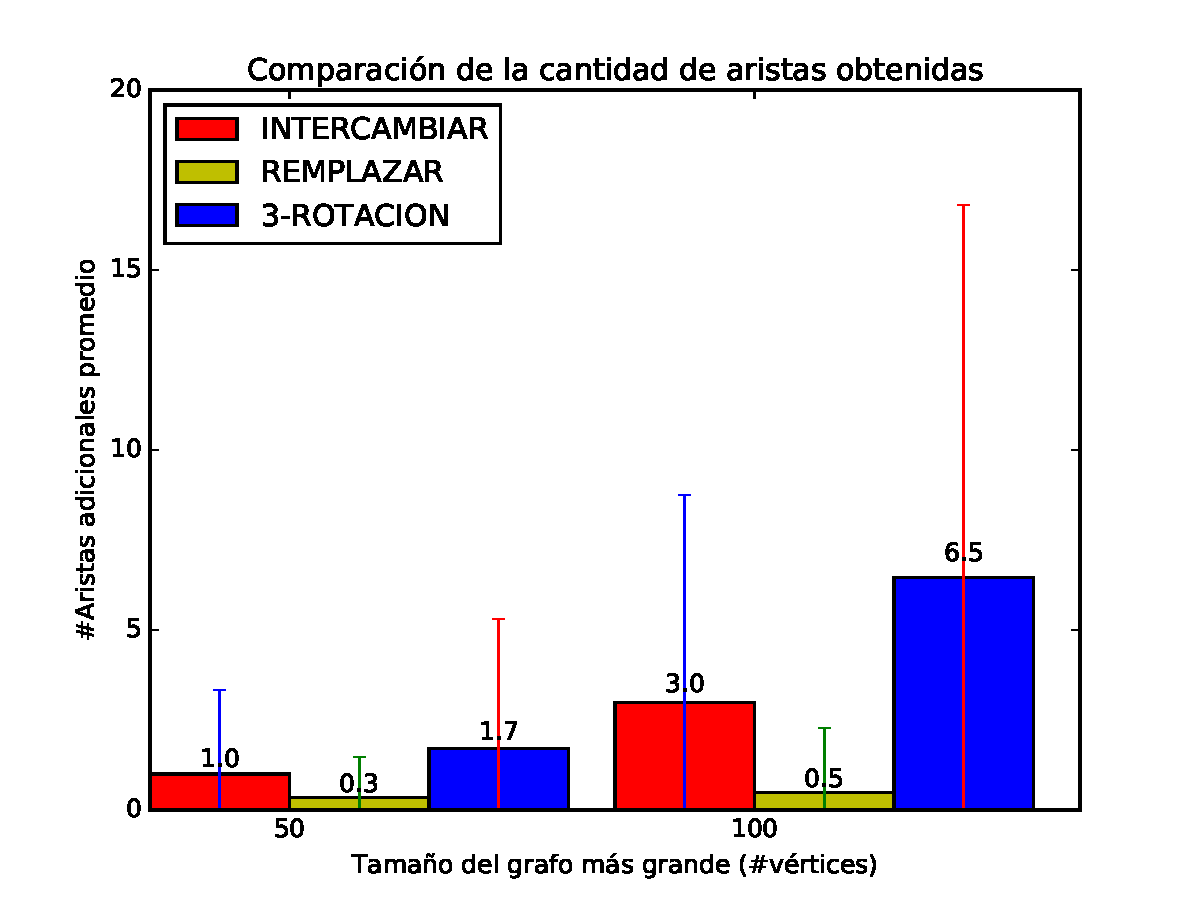
\includegraphics[width=1\textwidth]{graficos/problema_5/calidad0.pdf}
  \caption{}
  \label{fig:calidad1}
\end{minipage}%
\hspace{0.01\textwidth}
\begin{minipage}{0.49\textwidth}   
  \centering
    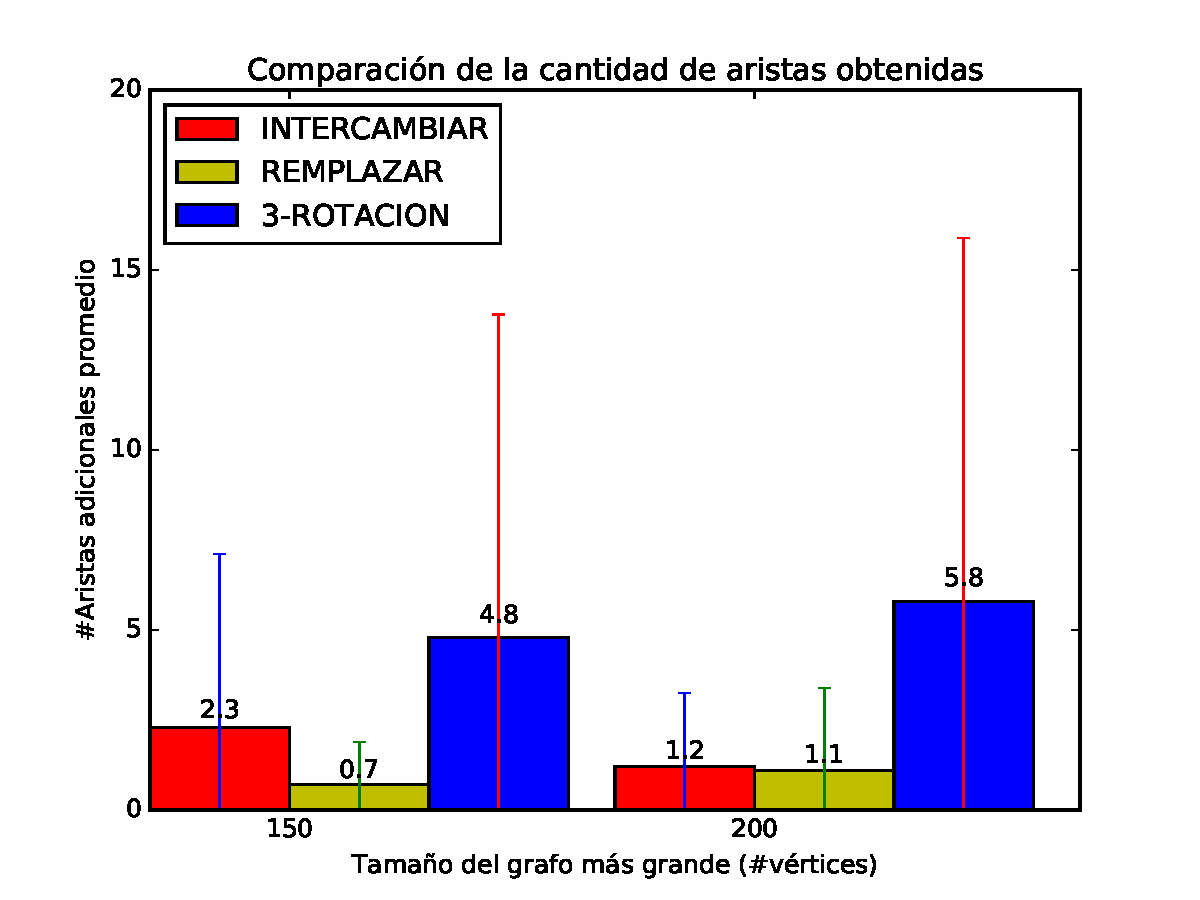
\includegraphics[width=1\textwidth]{graficos/problema_5/calidad2.pdf} 
  \caption{}
  \label{fig:calidad2}
\end{minipage}

\begin{minipage}{0.49\textwidth}
  \centering
    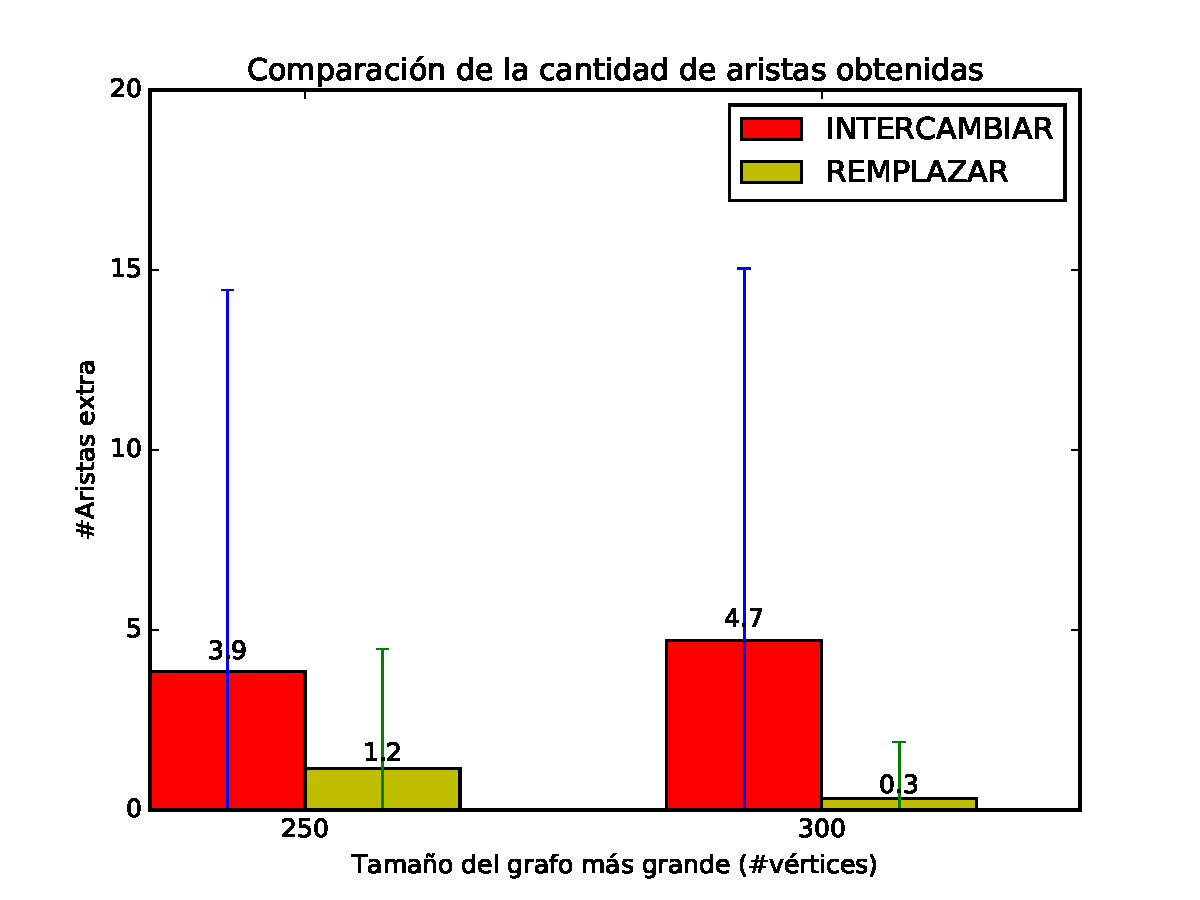
\includegraphics[width=1\textwidth]{graficos/problema_5/calidad4.pdf}
  \caption{}
  \label{fig:calidad3}
\end{minipage}%
\end{figure}

En lo gráficos de arriba puede verse una comparación de la calidad de los tres algoritmos, entendiendo a esta como la diferencia en la cantidad de aristas encontradas en promedio por cada uno. Lo primero que puede notarse observando las figuras \ref{fig:calidad1} y \ref{fig:calidad2} es la clara ventaja de 3-ROTACION sobre las otras heurísticas, tanto en el valor promedio como en los máximos alcanzados. Notar, sin embargo, que la razón por la que la calidad de este algoritmo no se grafica en la figura \ref{fig:calidad3} es que, como veremos a continuación, consume mucho más tiempo que sus competidores, por lo que muestrearlo para grafos de tamaño 250 y 300 resultaba ya muy costoso. Sin embargo, podemos ver que la ligera tendencia de superioridad de INTERCAMBIAR sobre REMPLAZAR, que se aprecia  en las primeras dos figuras, se mantiene (e incluso se acentúa) en la tercera. Como INTERCAMBIAR es un caso particular de 3-ROTACION está claro que entonces este último siempre debe seral menos tan bueno, lo que nos permite deducir que 3-ROTACION sigue siendo la mejor opción en calidad.

Ahora bien, como dijimos antes 3-ROTACION es cara temporalmente. En las figuras \ref{fig:tiempo1} y \ref{fig:tiempo2} se ve claramente como este algoritmo está órdenes de magnitud por encima de los otros dos en cuanto a tiempo utilizado se refiere. Nótese que fue necesario recurrir a la escala logarítmica pues de lo contrario INTERCAMBIAR y REMPLAZAR hubieran resultado indistinguibles por esta diferencia de órdenes.  Notar que entre estas dos heurísticas no hay una diferencia tan significativa, aunque si nos guiamos por estas dos figuras pareciera que INTERCAMBIAR tiende a consumir un poco más de tiempo. No obstante, la figura \ref{fig:tiempo3} viene a romper esta tendencia. 

Esta aparente contradicción en la tendencia podemos atribuírsela parcialmente a no tener un mayor número de muestras; en general, en términos amortizados podríamos esperar que estén en el mismo orden. Inicialmente no hay una razón para pensar que una tenga que ser más rápida que la otra en todos los casos. Mientras que por un lado INTERCAMBIAR solo depende de $n_1$, REMPLAZAR también lo hace de $n_2-n_1$, como vimos en la subsección de complejidad. Esto implica que el costo de las iteraciones será mayor para REMPLAZAR cuando dicha diferencia sea superior a $n_1$, y caso contrario cuando no lo sea. Aunque claro, también hay que tener en cuenta la cantidad de iteraciones que se realizan, lo que resulta poco predecible.  

\begin{figure}[H]
\centering
\begin{minipage}{0.49\textwidth}
  \centering
    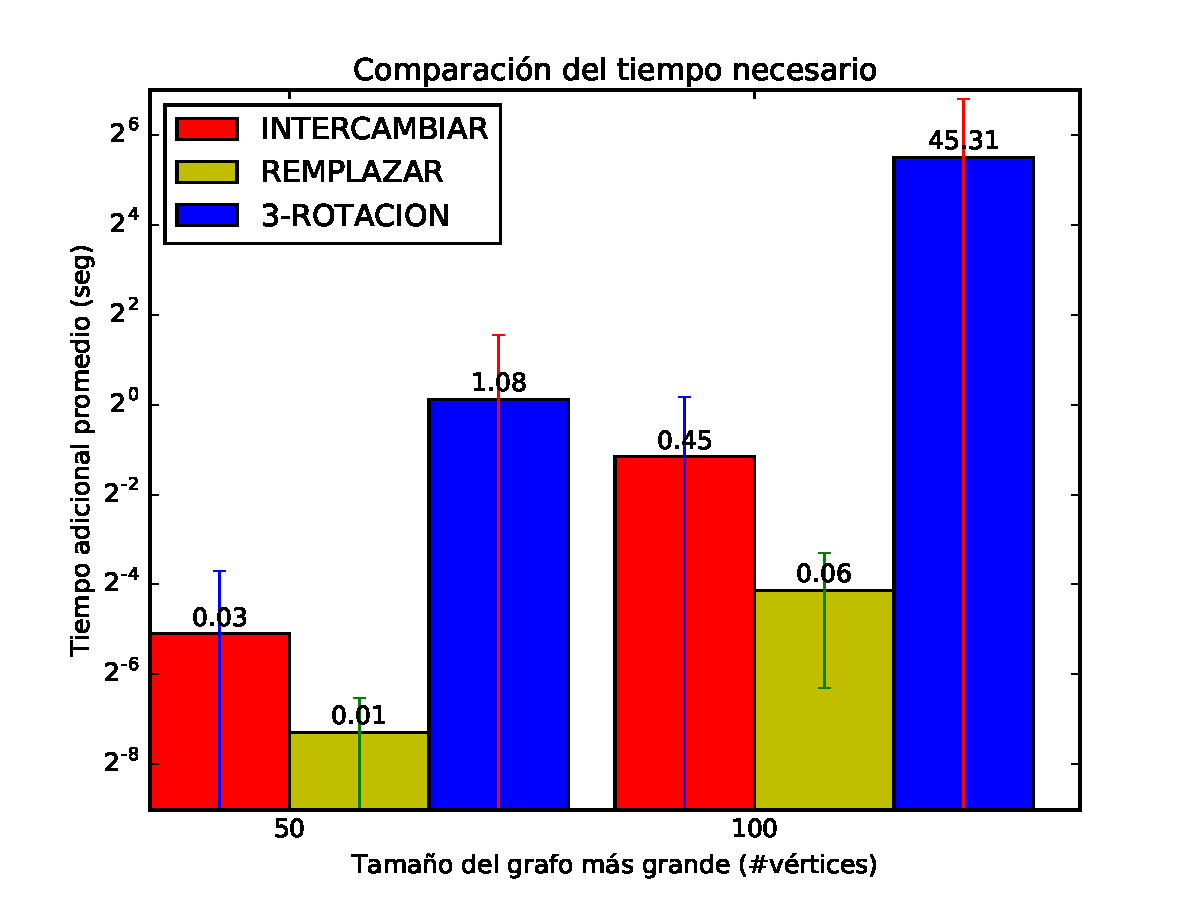
\includegraphics[width=1\textwidth]{graficos/problema_5/tiempo0.pdf}
  \caption{}
  \label{fig:tiempo1}
\end{minipage}%
\hspace{0.01\textwidth}
\begin{minipage}{0.49\textwidth}   
  \centering
    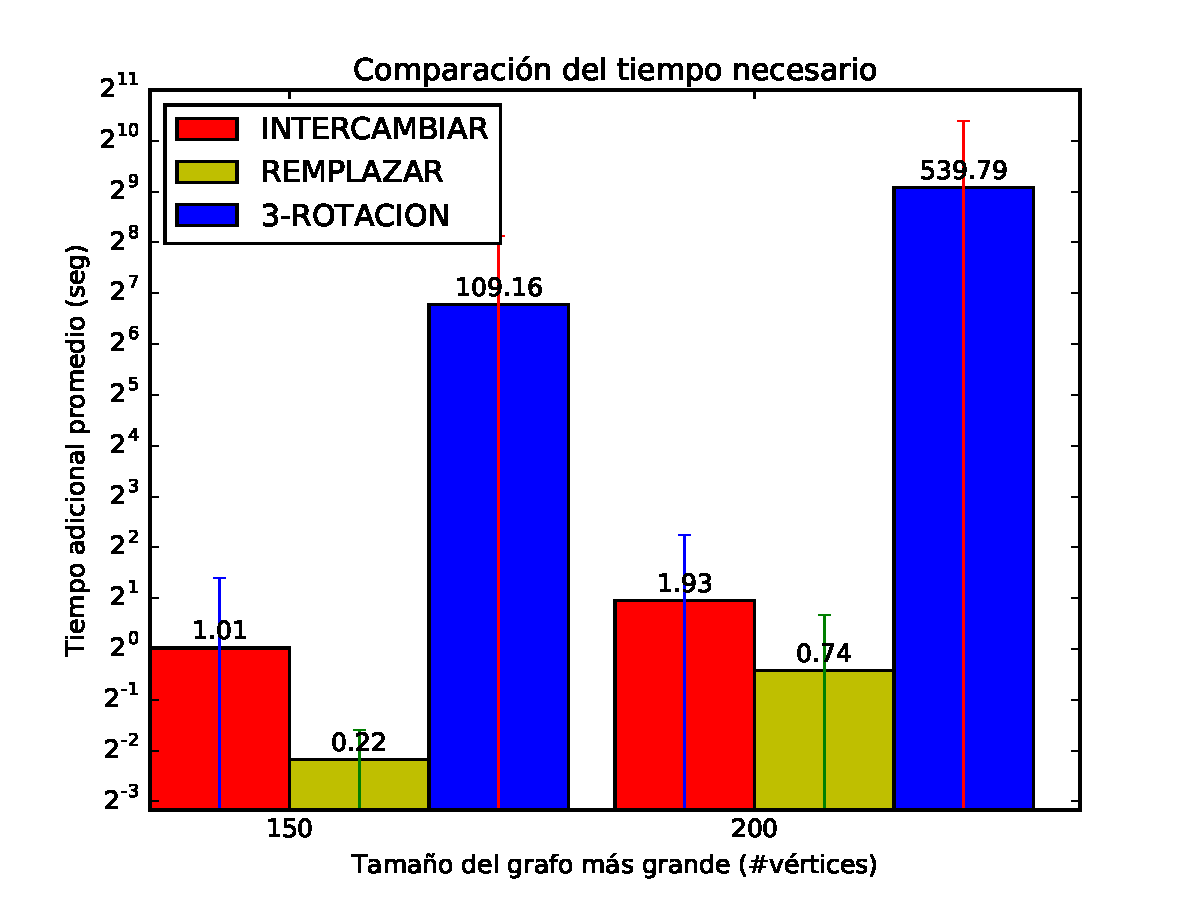
\includegraphics[width=1\textwidth]{graficos/problema_5/tiempo2.pdf} 
  \caption{}
  \label{fig:tiempo2}
\end{minipage}

\begin{minipage}{0.49\textwidth}
  \centering
    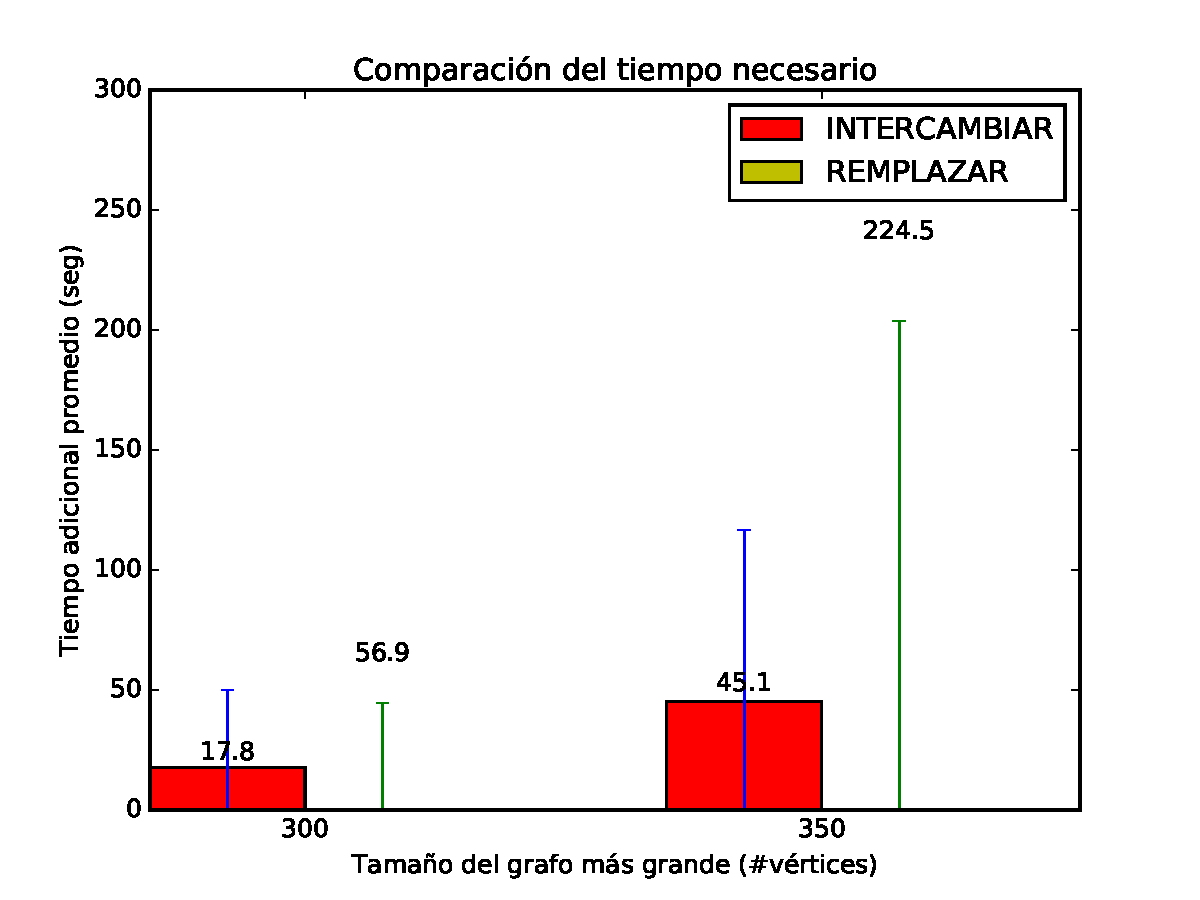
\includegraphics[width=1\textwidth]{graficos/problema_5/tiempo4.pdf}
  \caption{}
  \label{fig:tiempo3}
\end{minipage}%
\end{figure}

Finalmente veamos las últimas tres figuras, que son quizás las más relevantes pues nos permiten ver la relación calidad/tiempo. Sin demasiadas sorpresas, 3-ROTACION que había mostrado ser el mejor calidad tenía en términos relativos (aunque sin grandes diferencias en términos absolutos) pero también el marcadamente peor en cuanto a tiempos, da pobres resultados para esta estadística. Nuevamente tenemos resultados contradictorios entre las otras dos heurísticas, sin embargo vemos que son coherentes con los resultados obtenidos para los tiempos. 

En definitiva no parece haber un claro ganador entre estas dos alternativas. Ahora bien si aceptamos el hecho de que en general no podemos determinar que una de las dos siempre va a ser más rápida, estando bastante parejas en este apartado, sí pudimos ver que INTERCAMBIAR resultaba más robusta en cuanto a la cantidad de aristas encontradas, por lo que parece una decisión razonable quedarnos con esta heurística para el caso general. 

\begin{figure}[H]
\centering
\begin{minipage}{0.49\textwidth}
  \centering
    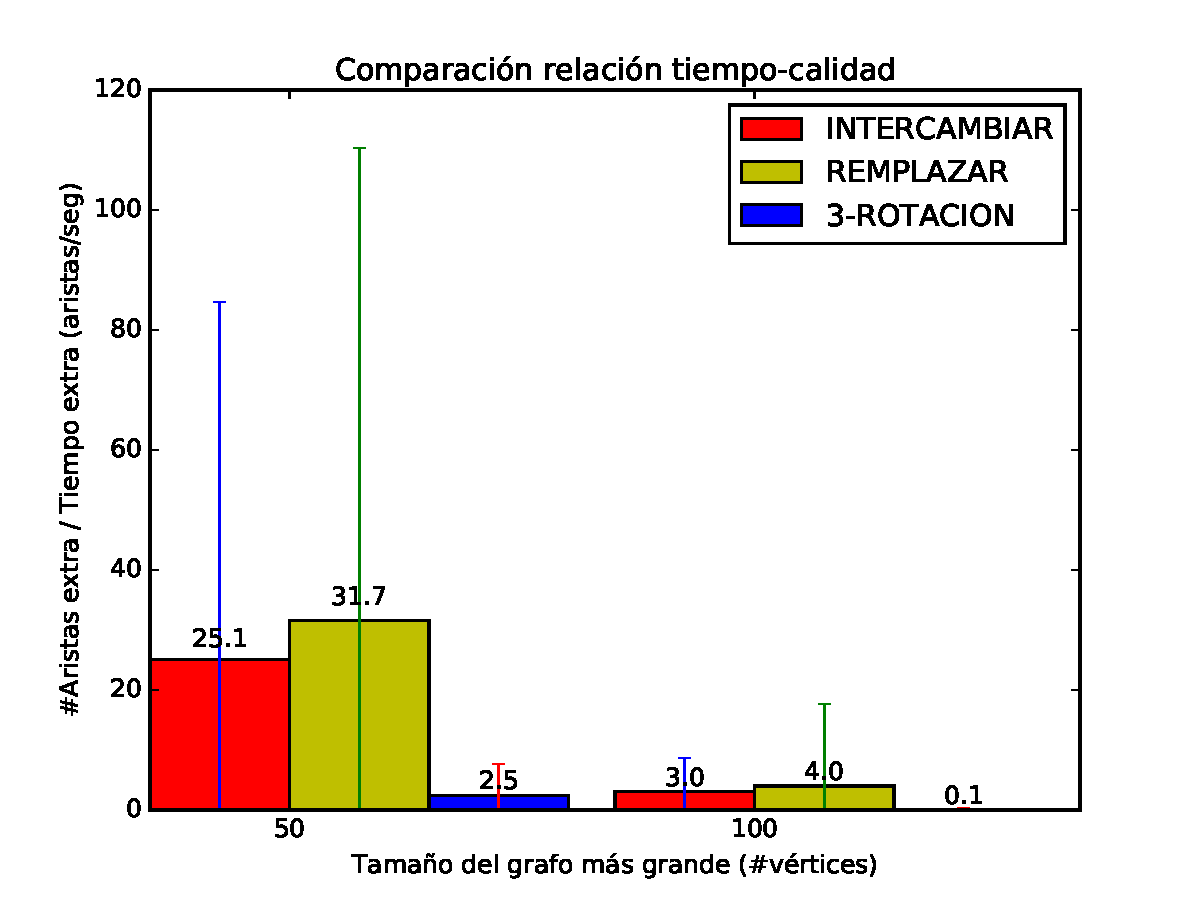
\includegraphics[width=1\textwidth]{graficos/problema_5/cociente1-0.pdf}
  \caption{}
  \label{fig:cociente1}
\end{minipage}%
\hspace{0.01\textwidth}
\begin{minipage}{0.49\textwidth}   
  \centering
    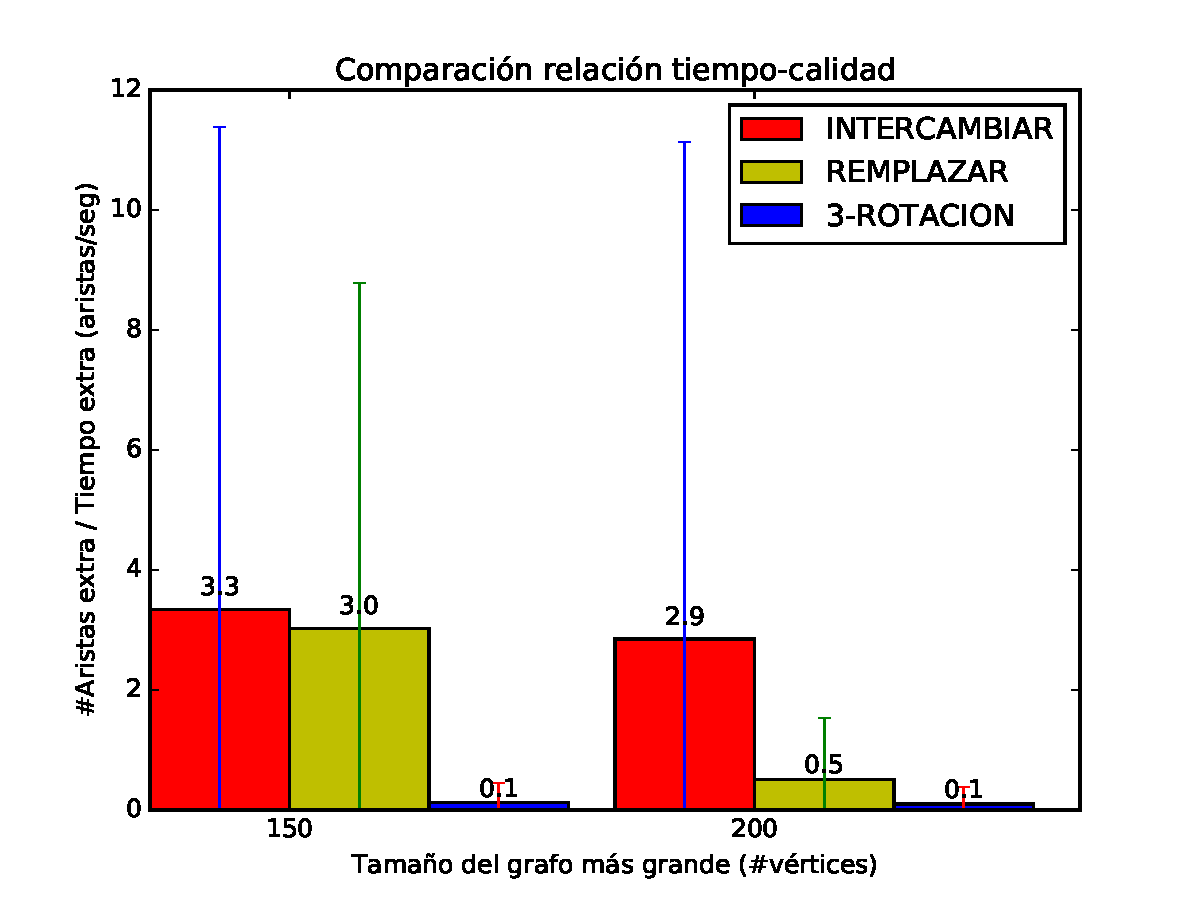
\includegraphics[width=1\textwidth]{graficos/problema_5/cociente1-2.pdf} 
  \caption{}
  \label{fig:cociente2}
\end{minipage}

\begin{minipage}{0.49\textwidth}
  \centering
    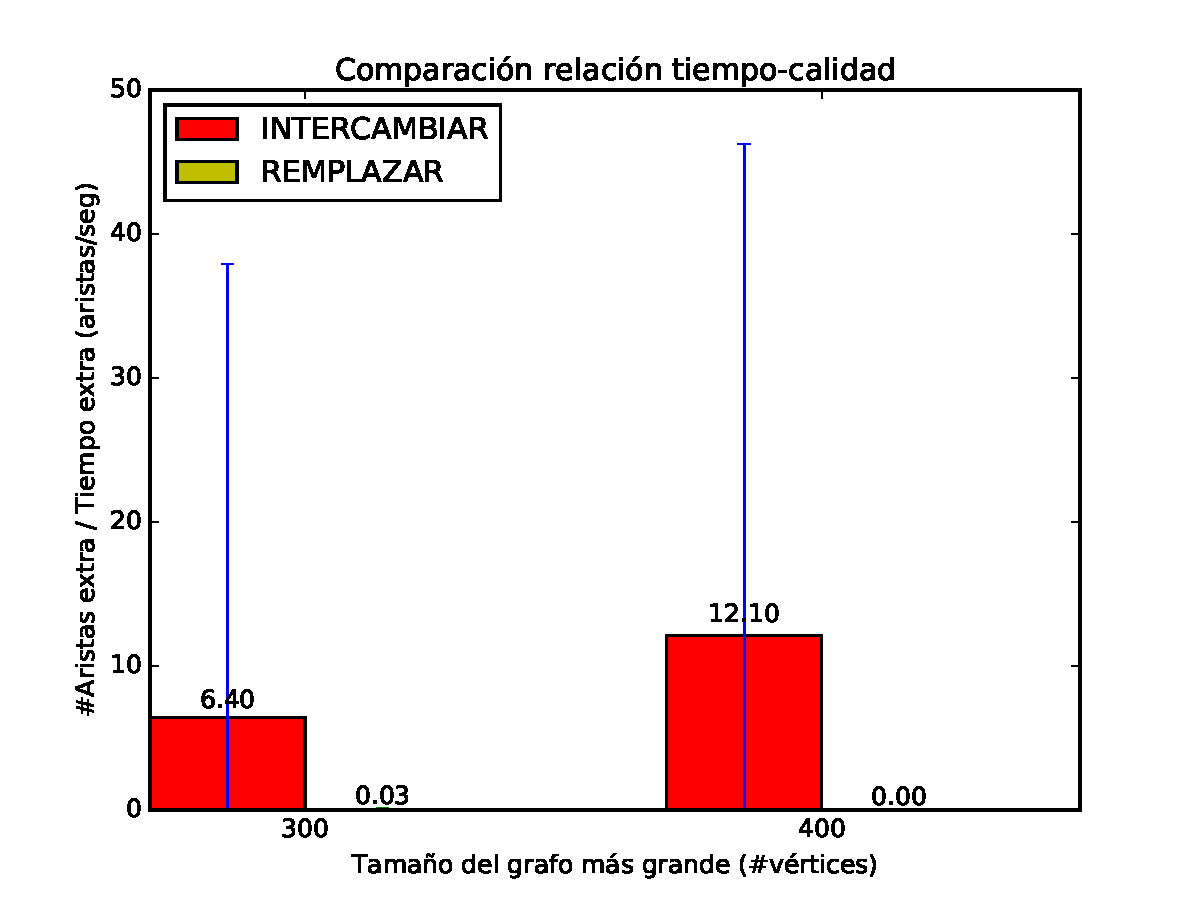
\includegraphics[width=1\textwidth]{graficos/problema_5/cociente0-4.pdf}
  \caption{}
  \label{fig:cociente3}
\end{minipage}%

\end{figure}



